\chapter{Implementacija i korisničko sučelje}
		
		
		\section{Korištene tehnologije i alati}
		
			%\textbf{\textit{dio 2. revizije}}
			Kako bi što više ubrzali i olakšali komunikaciju među članovima tima, koristili smo dvije aplikacije: \underline{Whatsapp}\footnote{\url{https://www.whatsapp.com/}} i \underline{Discord}\footnote{\url{https://discord.com/}}. Kako bismo se dodatno upoznali s tehnologijom koja se često koristi u praksi, koristili smo i platformu \underline{Jira}\footnote{\url{https://www.atlassian.com/software/jira}} za organizaciju i podjelu zadataka na članove tima putem zadataka (engl. task) na Kanban ploči. Kao distribuirani sustav za upravljanje izvornim kodom koristili smo \underline{Git}\footnote{\url{https://git-scm.com/}}, a sami repozitorij projekta dostupan je na platformi \underline{Gitlab}\footnote{\url{https://gitlab.com/}}\\

            Za razvoj korisničkog sučelja tj. frontenda općenito, korišteni su markup jezik \underline{HTML}\footnote{\url{https://en.wikipedia.org/wiki/HTML}}, stilski jezik \underline{CSS}\footnote{\url{https://en.wikipedia.org/wiki/CSS}}, programski jezik \underline{Javascript}\footnote{\url{https://www.javascript.com/}} i \underline{React.js}\footnote{\url{https://reactjs.org/}}. React.js knjižnica je pisana u jeziku Javascript koja omogućava jednostavan i relativno brz razvoj komponenti koje je lako ponovno koristiti, a razvija ga primarno tvrtka Meta. Uz React.js, za razvoj robusnih i kvalitetnih komponenti, korišten je \underline{Material UI}\footnote{\url{https://mui.com/}} - open-source knjižnica React komponenti. Za pisanje koda u navedenim jezicima korišten je \underline{Visual Studio Code}\footnote{\url{https://code.visualstudio.com/}} - veoma popularan IDE (integrirana razvojna okolina) s velikim brojem opcionalnih ekstenzija koje služe kao pomoć pri razvoju. VSC razvija tvrtka Microsoft. \\

            \eject

            Za razvoj backenda korišten je programski jezik \underline{Java}\footnote{\url{https://www.java.com/en/}} - objektno orijentirani jezik korišten u brojnim aspektima razvoja programske potpore. Jezik Java razvija tvrtka Oracle. Uz to, korišten je \underline{Java Spring Boot}\footnote{\url{https://spring.io/projects/spring-boot}} - specijalizacija radnog okvira \underline{Java Spring}\footnote{\url{https://spring.io/}} razvijena s ciljem što bržeg, lakšeg i učinkovitijeg razvoja web aplikacija. Za pisanje koda u jeziku Java korišten je \underline{IntelliJ IDEA}\footnote{\url{https://www.jetbrains.com/idea/}} - integrirana razvojna okolina često korištena za razvoj programske potpore u jezicima Java i Kotlin. Intellij IDEA razvija tvrtka JetBrains. \\

            Za razvoj baze podataka korišten je sustav za upravljanje relacijskim bazama podataka \underline{PostgreSQL}\footnote{\url{https://www.postgresql.org/}}. Uz to, za lokalni razvoj i testiranje baze podataka korištena je aplikacija \underline{pgAdmin}\footnote{\url{https://www.pgadmin.org/}}. \\

            Za kreiranje potrebnih UML dijagrama korišten je alat \underline{Visual Paradigm Online}\footnote{\url{https://online.visual-paradigm.com/}} koji omogućava zajednički rad na dijagramima, time olakšavajući organizaciju i dijeljenje istih s članovima tima. Za razvoj dokumentacije korišten je markup jezik \underline{LaTeX}\footnote{\url{https://www.latex-project.org/}}, već navedena integrirana razvojna okolina Visual Studio Code i alat \underline{Overleaf}\footnote{\url{https://www.overleaf.com/}} koji omogućava online pisanje LaTeX koda.\\

            Frontend, backend i baza podataka pušteni su u pogon na platformi \underline{Render}\footnote{\url{https://render.com/}} koja omogućava besplatan i relativno jednostavan deploy aplikacija. Za uspješno puštanje u pogon backend koda, potrebno je pripremiti i \underline{Docker}\footnote{\url{https://www.docker.com/}} Container kako bi na istom mjestu bilo dostupno sve potrebno za uspješno puštanje backend-a u pogon. \\
		
			\eject 
		
	
		\section{Ispitivanje programskog rješenja}
			
			%\textbf{\textit{dio 2. revizije}}\\
			
			 Kako bismo što učinkovitije testirali naš sustav, testirali smo ispravnost rada pojedinih komponenti koristeći unit testove, ali i ispravnost rada čitavog sustava koristeći alat Selenium.
	
			
			\subsection{Ispitivanje komponenti}

                Za testiranje rada komponenti, napisano je i pokrenuto 9 unit testova. Testovi su pisani u programskom jeziku Java koristeći okvir za testiranje JUnit. Na slikama se nalazi kod samih testova, kao i dokaz da testovi prolaze (redak Tests passed). Uz to, vidljivo je i trajanje izvođenja testova.\\
                
                \subsubsection{Test 1}
                Prvim testom provjerava se valjanost zapisa o kategoriji pri dohvaćanju potkategorije - ako je dohvaćena potkategorija "Lutke", u dohvaćenom podatku trebao bi postojati i zapis o pripadnoj kategoriji - "Igračke". \underline{Test prolazi.}

                \begin{figure}[H]
				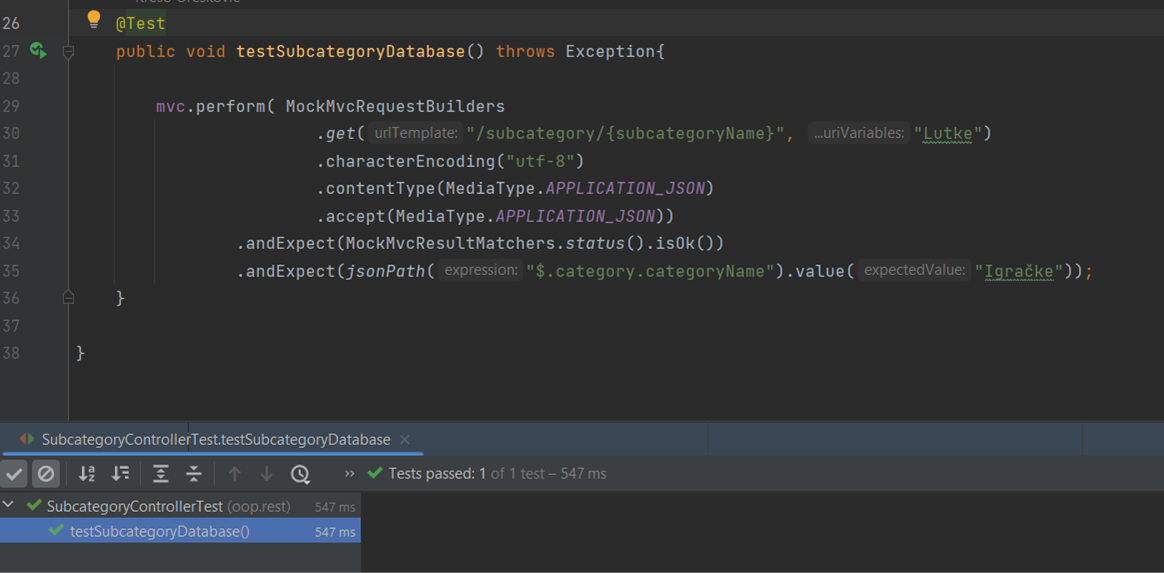
\includegraphics[]{slike/unit1.png}
				\centering
				\caption{Kod prvog unit testa}
				\label{fig:unit1}
			\end{figure}

                \eject

                \subsubsection{Test 2}
                Drugim testom provjerava se dolazi li do pogreške ako pri registraciji korisnik unese mail adresu koja je već unešena u bazi - očekivan je status "400 Bad Request". \underline{Test prolazi.}

                \begin{figure}[H]
				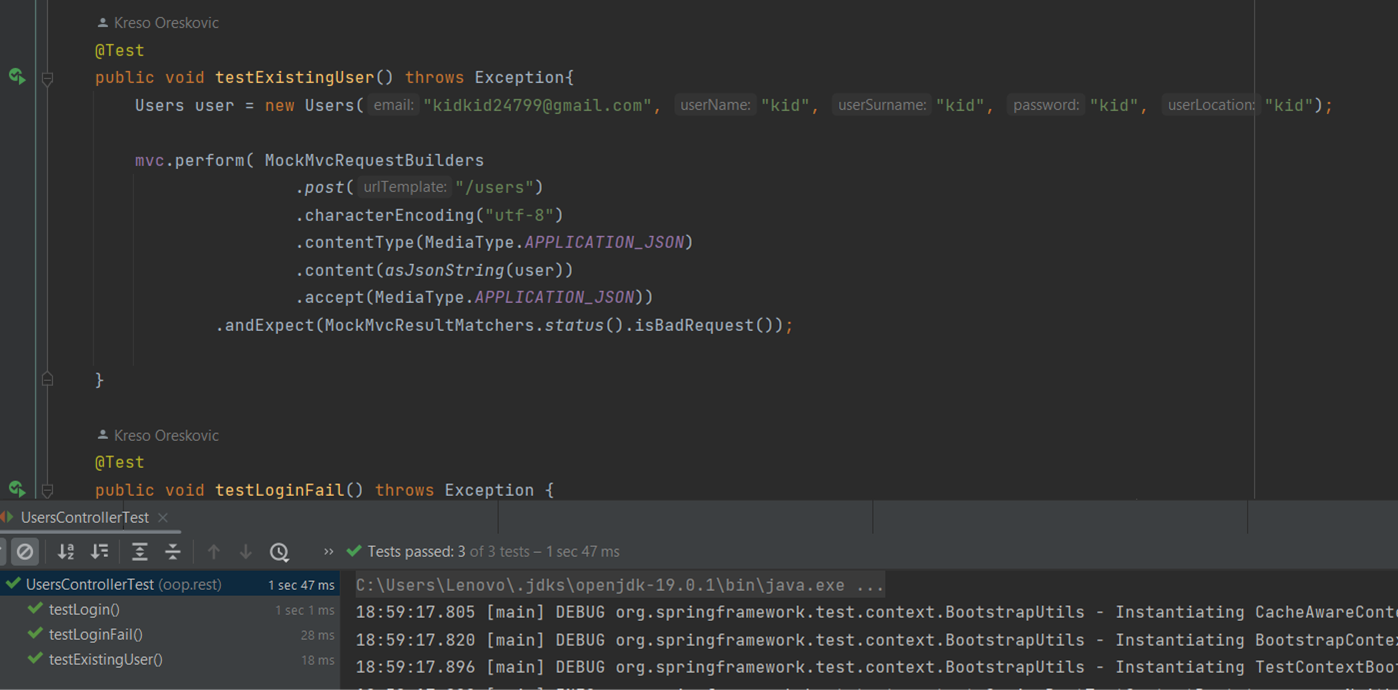
\includegraphics[scale=0.9]{slike/unit2.png}
				\centering
				\caption{Kod drugog unit testa}
				\label{fig:unit2}
			\end{figure}

                \subsubsection{Test 3}
                Trećim testom provjerava se dolazi li do pogreške ako pri loginu korisnik unese mail adresu za koju u bazi ne postoji zapis tj. podaci o korisniku. \underline{Test prolazi.}

                \begin{figure}[H]
				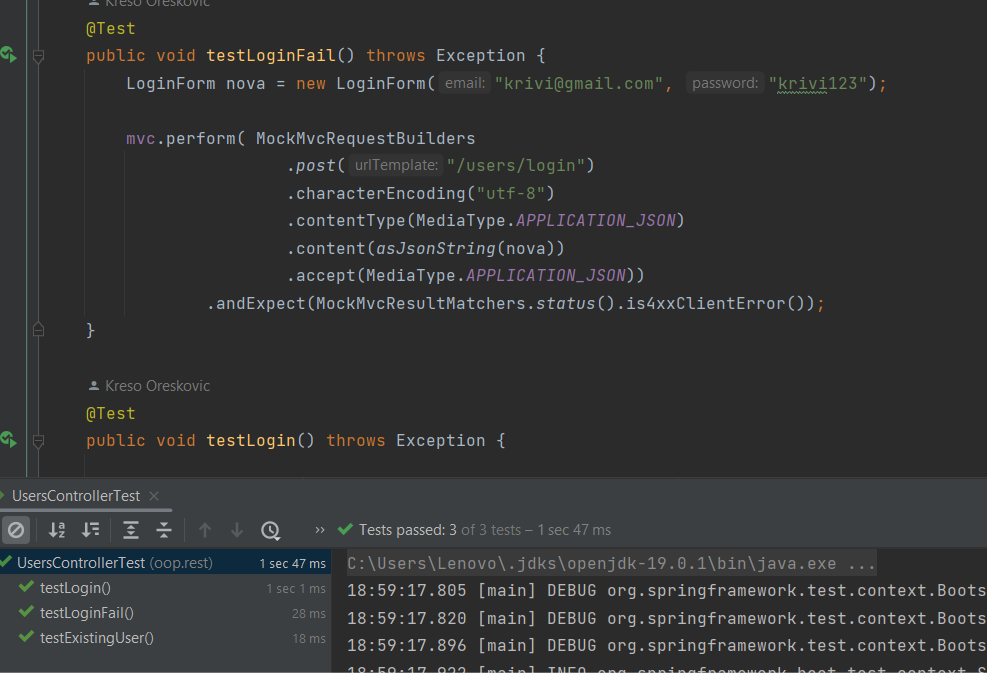
\includegraphics[scale=0.8]{slike/unit3.png}
				\centering
				\caption{Kod trećeg unit testa}
				\label{fig:unit3}
			\end{figure}

                \eject
            
                \subsubsection{Test 4}
                Četvrtim testom provjerava se uspješnost logina korisnika za kojeg u bazi postoje podaci. \underline{Test prolazi.}

                \begin{figure}[H]
				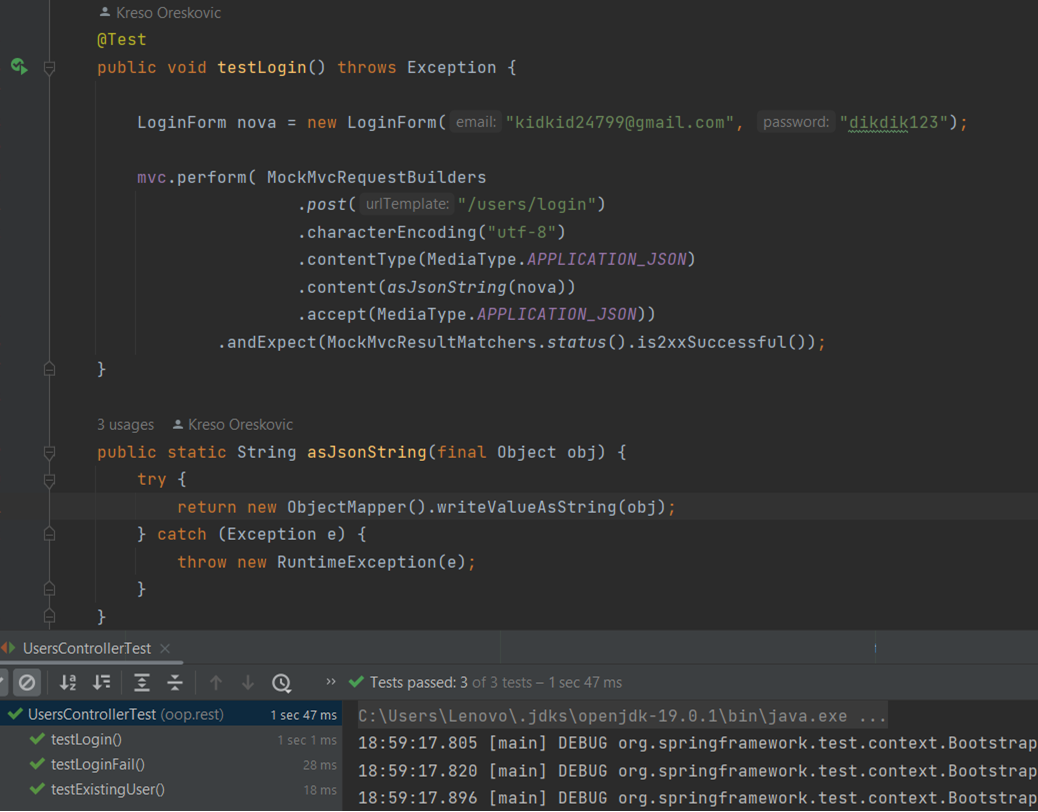
\includegraphics[]{slike/unit4.png}
				\centering
				\caption{Kod četvrtog unit testa}
				\label{fig:unit4}
			\end{figure}

                \subsubsection{Test 5}
                Petim testom provjerava se uspješnost stvaranja donacije. \underline{Test prolazi.}

                \begin{figure}[H]
				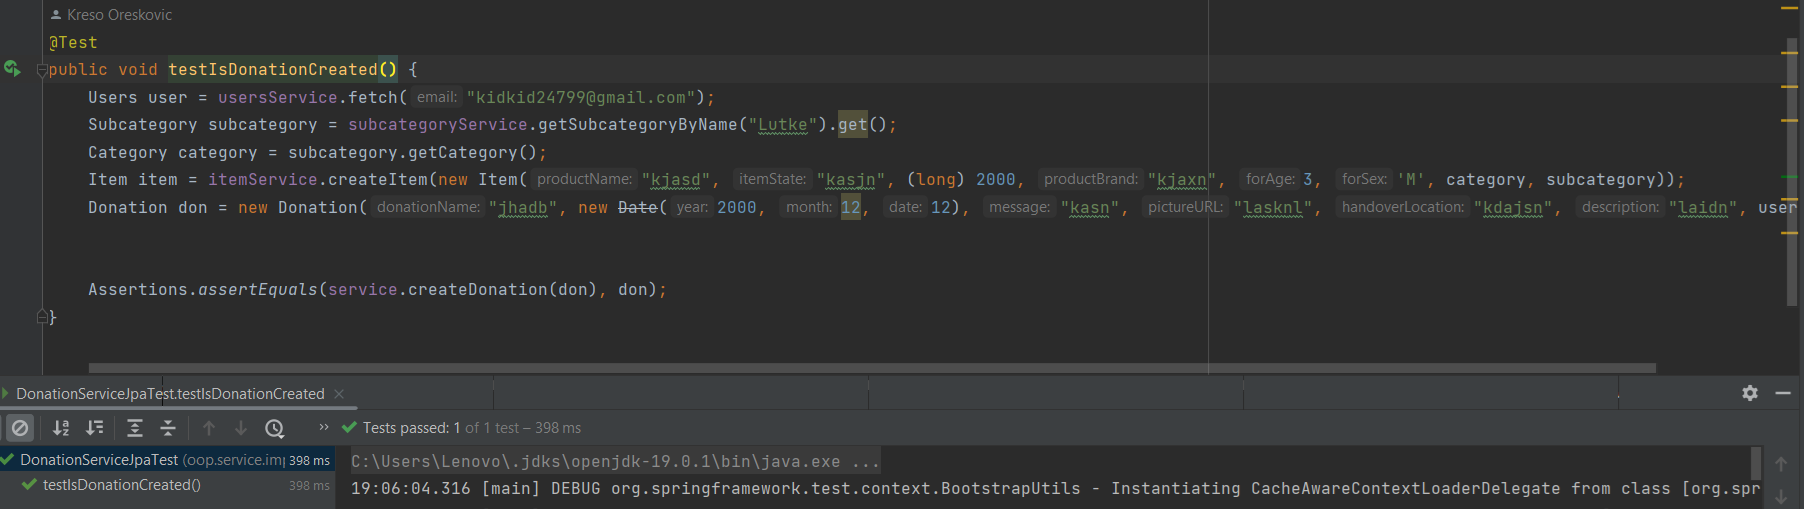
\includegraphics[]{slike/unit5.png}
				\centering
				\caption{Kod petog unit testa}
				\label{fig:unit5}
			\end{figure}

                \subsubsection{Testovi 6, 7}
                Šestim testom provjerava se uspješnost ažuriranja podataka o predmetu. \underline{Test prolazi.}
                Sedmim testom provjerava se uspješnost brisanja predmeta iz baze podataka, kao i dolazi li do "custom" pogreške "EntityMissingException" pri pokušaju dohvaćanja izbrisanog predmeta. \underline{Test prolazi.}

                \begin{figure}[H]
				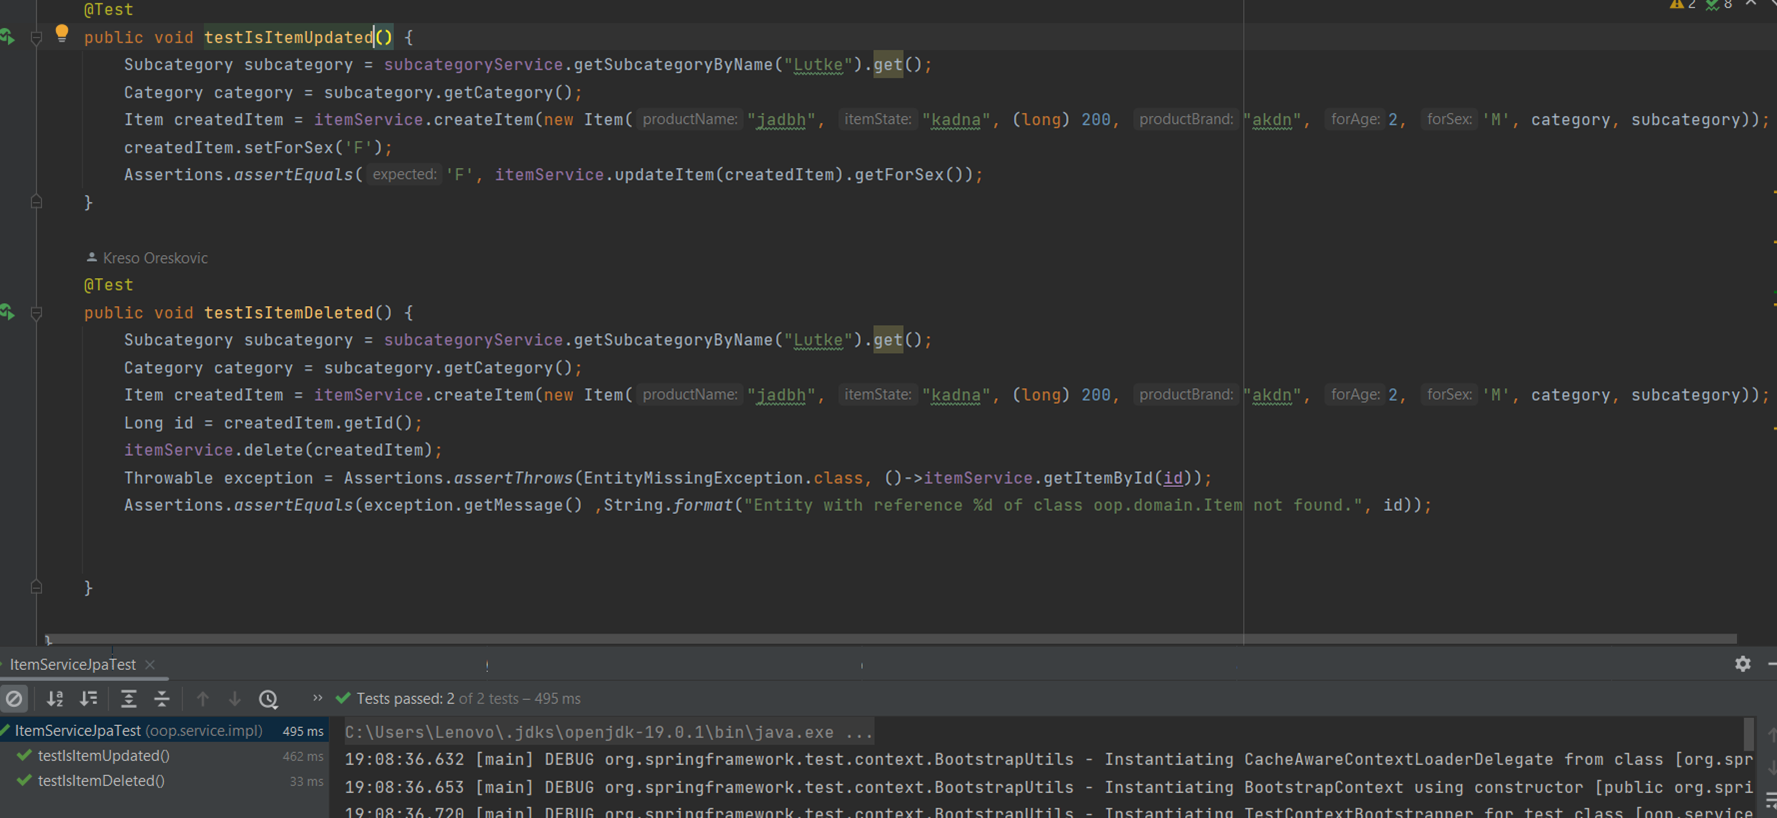
\includegraphics[]{slike/unit6.png}
				\centering
				\caption{Kod šestog i sedmog unit testa}
				\label{fig:unit67}
			\end{figure}

                \subsubsection{Testovi 8, 9}
                Osmim testom provjerava se postoji li admin račun u bazi podataka. \underline{Test prolazi.}
                Devetim testom provjerava se dolazi li do "custom" pogreške "EntityMissingException" pri pokušaju dohvaćanja nepostojećeg korisnika. \underline{Test prolazi.}

                \begin{figure}[H]
				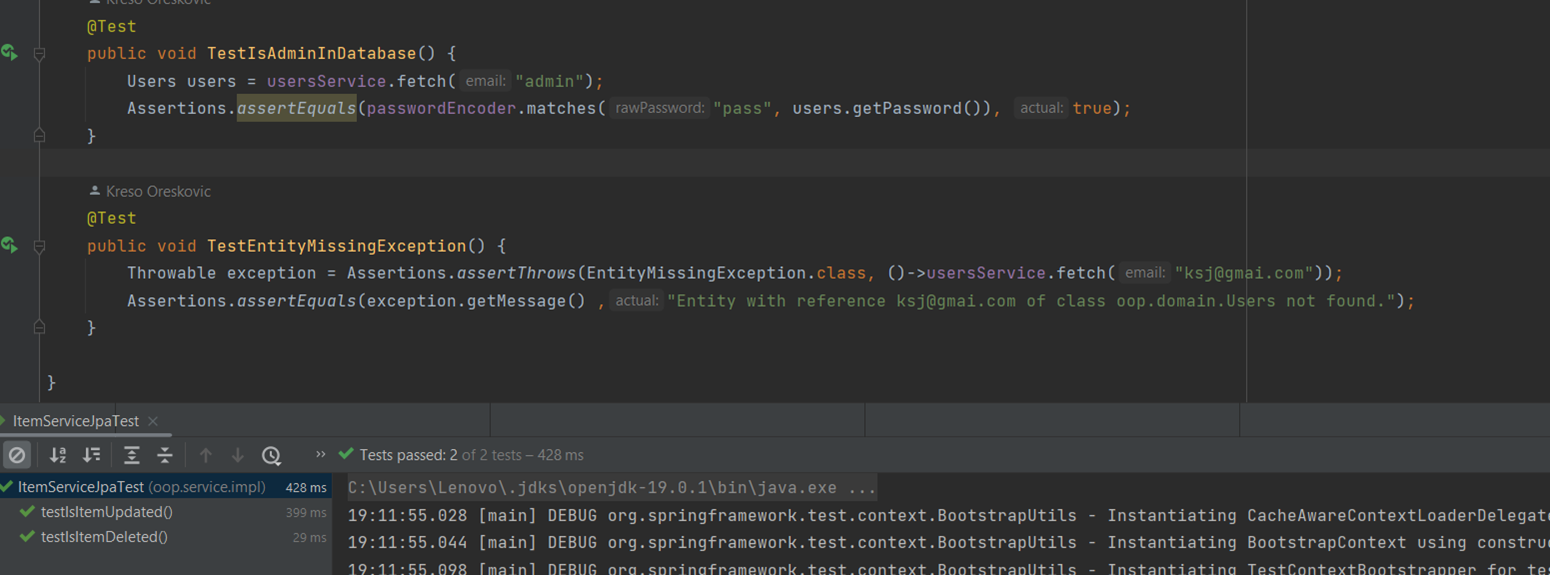
\includegraphics[]{slike/unit7.png}
				\centering
				\caption{Kod osmog i devetog unit testa}
				\label{fig:unit89}
			\end{figure}

                \eject
                
			%\textit{Potrebno je provesti ispitivanje jedinica (engl. unit testing) nad razredima koji implementiraju temeljne funkcionalnosti. 
			%Razraditi \textbf{minimalno 6 ispitnih slučajeva} u kojima će se ispitati redovni slučajevi, rubni uvjeti te izazivanje pogreške (engl. exception throwing). 
			%Poželjno je stvoriti i ispitni slučaj koji koristi funkcionalnosti koje nisu implementirane. 
			%Potrebno je priložiti izvorni kôd svih ispitnih slučajeva te prikaz rezultata izvođenja ispita u razvojnom okruženju (prolaz/pad ispita). }

        
			
			
			
			\subsection{Ispitivanje sustava}

                Za testiranje rada cjelovitog sustava, korišteni su alati Selenium Webdriver i Selenium IDE. Selenium Webdriver omogućava pisanje testova cjelovitog sustava koristeći proizvoljan programski jezik, kao i integraciju tih testova s unit testovima napisanim za testiranje rada pojedinačnih komponenti. S druge strane, Selenium IDE korisnicima omogućava generiranje testova cjelovitog sustava snimanjem svojih akcija i ponavljanjem tih akcija. \\
                
                U našem testiranju, testirali smo funkcionalnosti aplikacije koja je već puštena u pogon (engl. deployana). Pritom smo za jednostavnije funkcionalnosti ručno pisali testove u programskom jeziku Java, dok smo za neke od složenijih funkcionalnosti snimili akcije koristeći alat Selenium IDE. Na slikama vidljiv je kod testova pisanih koristeći Selenium Webdriver, kao i akcije snimljene alatom Selenium IDE. Testovi pisani u programskom jeziku Java izvršeni su zajedno, a rezultat njihovog izvođenja prikazan je na zasebnoj slici. 

                \subsubsection{Test 1}
                Prvim testom provjerava se registracija koristeći već unesenu mail adresu tj. adresu za koju u bazi već postoji zapis o korisniku. Očekivani rezultat izvođenja testa je da ne dolazi do preusmjeravanja na stranicu s prikazom aktivnih oglasa, već je i dalje prikazana stranica za registraciju (s porukom o neuspješnoj registraciji). \underline{Test prolazi.}

                \begin{figure}[H]
				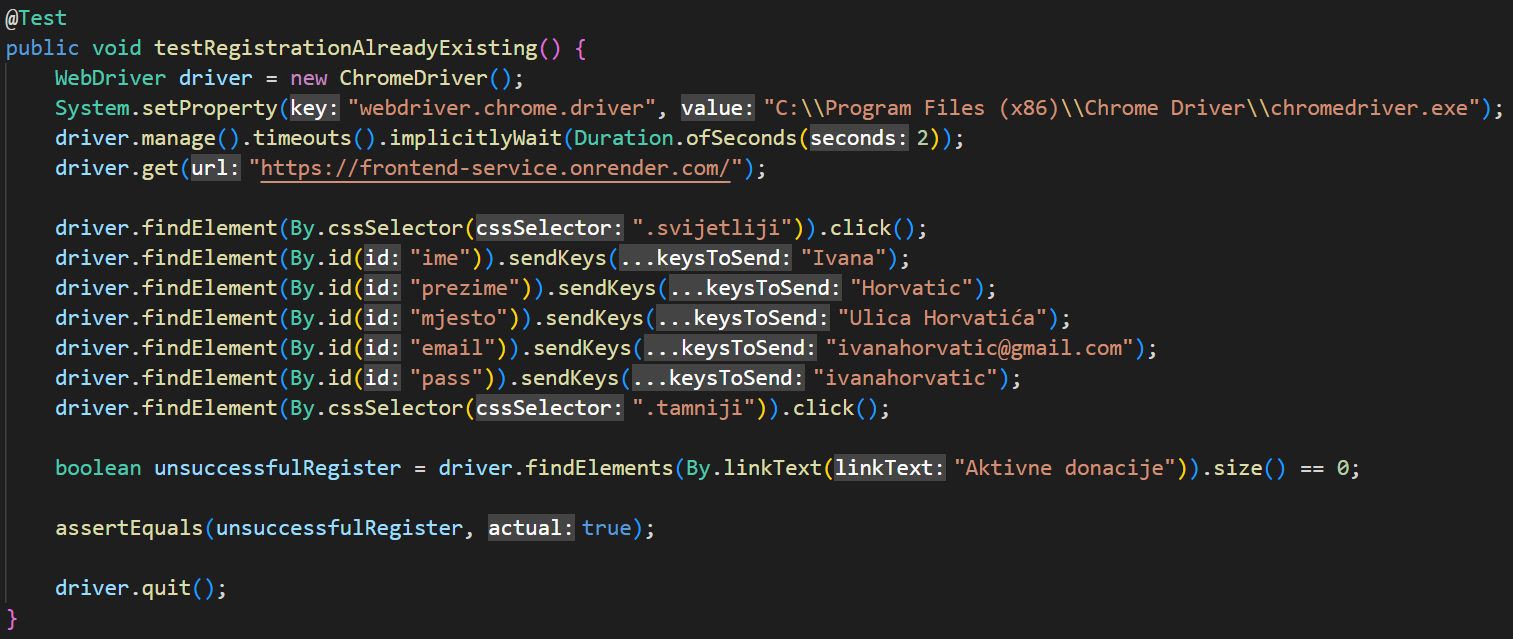
\includegraphics[scale=0.55]{slike/selenium1.png}
				\centering
				\caption{Kod prvog Selenium testa}
				\label{fig:selenium1}
			\end{figure}

                \subsubsection{Test 2}
                Drugim testom provjerava se registracija koristeći ispravne podatke tj. podatke za koje u bazi do sada ne postoji zapis o korisniku. Očekivani rezultat izvođenja testa je da dolazi do preusmjeravanja na stranicu s prikazom aktivnih oglasa koja u zaglavlju ima poveznice na ostale dijelove stranice. \underline{Test prolazi.}

                \begin{figure}[H]
				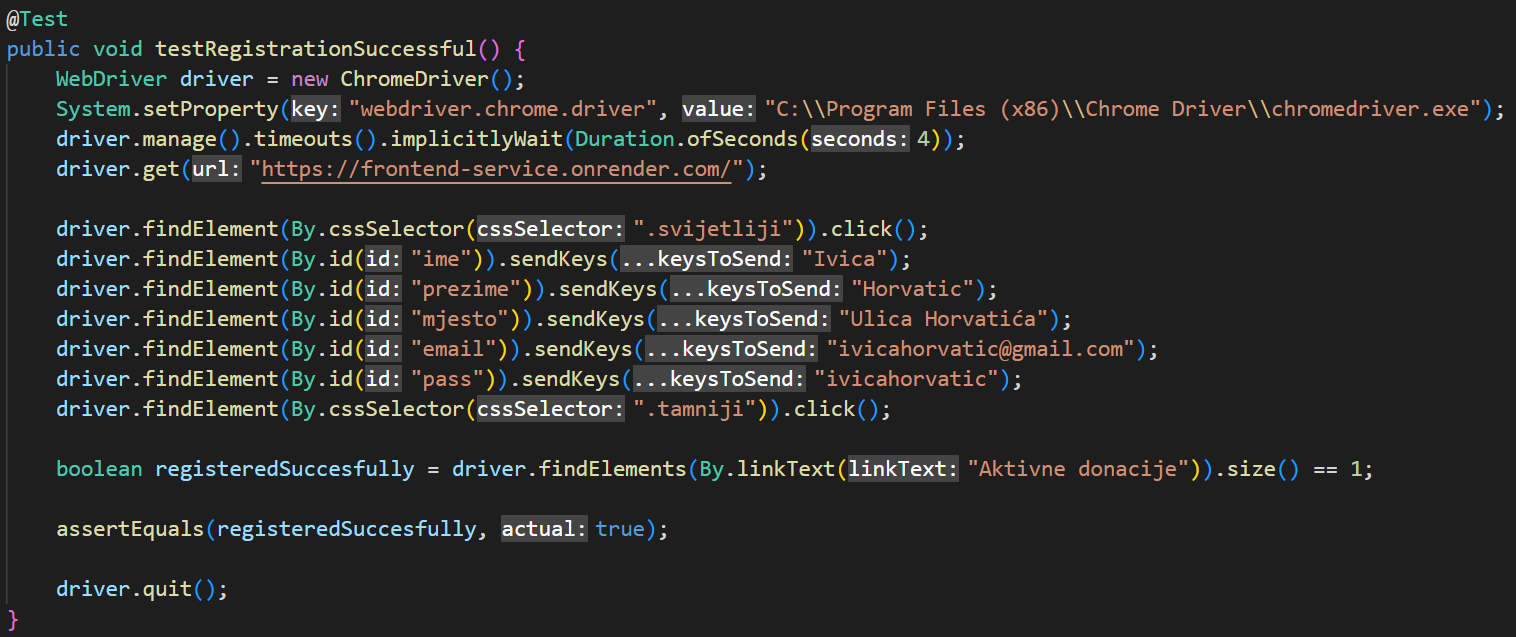
\includegraphics[scale=0.55]{slike/selenium2.png}
				\centering
				\caption{Kod drugog Selenium testa}
				\label{fig:selenium2}
			\end{figure}

                \subsubsection{Test 3}
                Trećim testom provjerava se login korisnika koristeći neispravne podatke (kombinacija ispravna mail adresa, neispravna lozinka korisnika). Očekivani rezultat izvođenja testa je da ne dolazi do preusmjeravanja na stranicu s prikazom aktivnih oglasa, već je i dalje prikazana stranica za login (s porukom o neuspješnoj prijavi). \underline{Test prolazi.}

                \begin{figure}[H]
				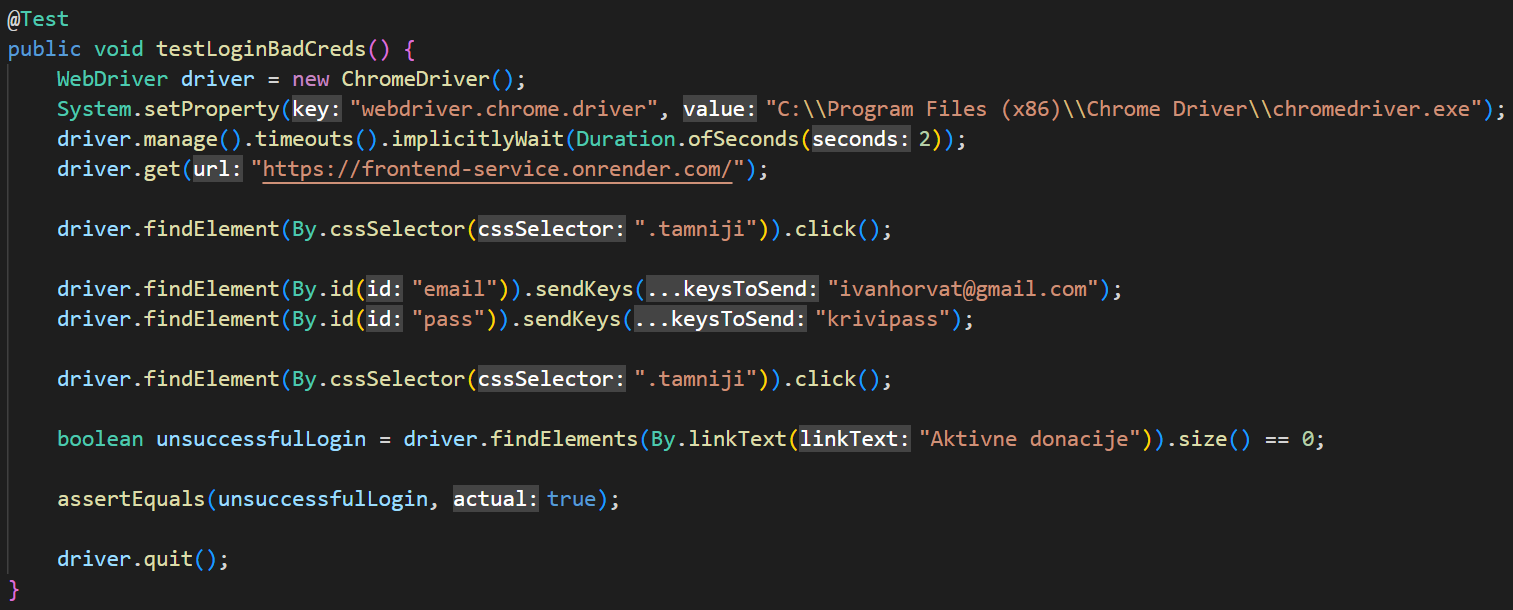
\includegraphics[scale=0.55]{slike/selenium3.png}
				\centering
				\caption{Kod trećeg Selenium testa}
				\label{fig:selenium3}
			\end{figure}

                \subsubsection{Test 4}
                Četvrtim testom provjerava se login korisnika koristeći ispravne podatke (ispravna mail adresa, ispravna lozinka korisnika). Očekivani rezultat izvođenja testa je da dolazi do preusmjeravanja na stranicu s prikazom aktivnih oglasa koja u zaglavlju ima poveznice na ostale dijelove stranice. \underline{Test prolazi.}

                \begin{figure}[H]
				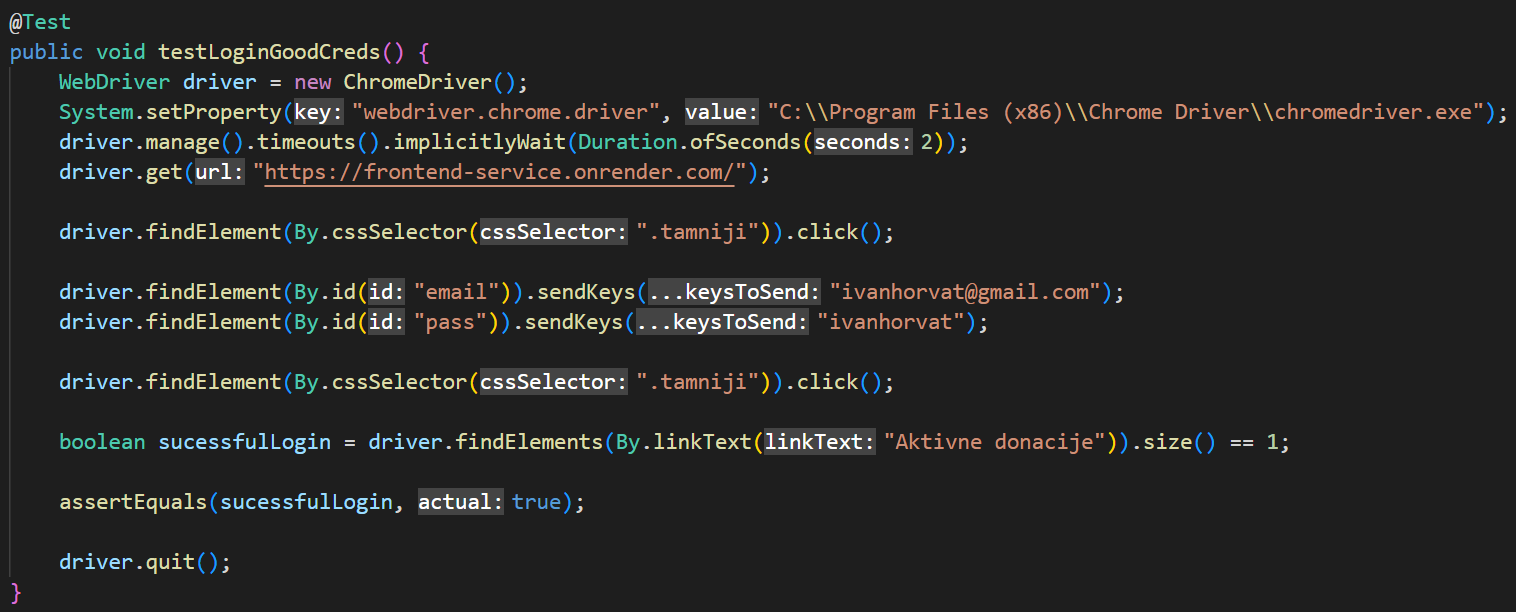
\includegraphics[scale=0.55]{slike/selenium4.png}
				\centering
				\caption{Kod četvrtog Selenium testa}
				\label{fig:selenium4}
			\end{figure}

                \subsubsection{Rezultati izvođenja Selenium testova}
                Na slici 5.12 prikazani su rezultati izvođenja do sada opisanih testova. Sva četiri testa uspješno prolaze, a na slici je prikazano i trajanje pojedinih testova.

                \begin{figure}[H]
				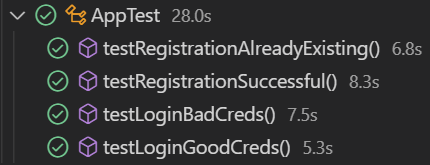
\includegraphics[]{slike/selenium_results.png}
				\centering
				\caption{Rezultati izvođenja Selenium testova}
				\label{fig:seleniumResults}
			\end{figure}

                \eject

                \subsubsection{Test 5}
                Na slici 5.13 prikazane su akcije snimljene koristeći alat Selenium IDE. Alat Selenium IDE korišten je kako bi se preglednije prikazale potrebne akcije - kod za testiranje složenih funkcionalnosti dugačak je i nepregledniji od ovakvog prikaza. Testirano je dodavanje nove kategorije. Kako bi se dodala nova kategorija, korisnik se mora prijaviti koristeći admin podatke. Tijekom provođenja testa, ti su podaci već bili pohranjeni u pregledniku pa je bilo dovoljno kliknuti na gumb za prijavu. Nakon uspješne prijave, dolazimo do stranice za dodavanje kategorija i potkategorija te pokušavamo stvoriti novu kategoriju proizvoljnog imena. \underline{Test prolazi.}

                \begin{figure}[H]
                \makebox[\textwidth][c]{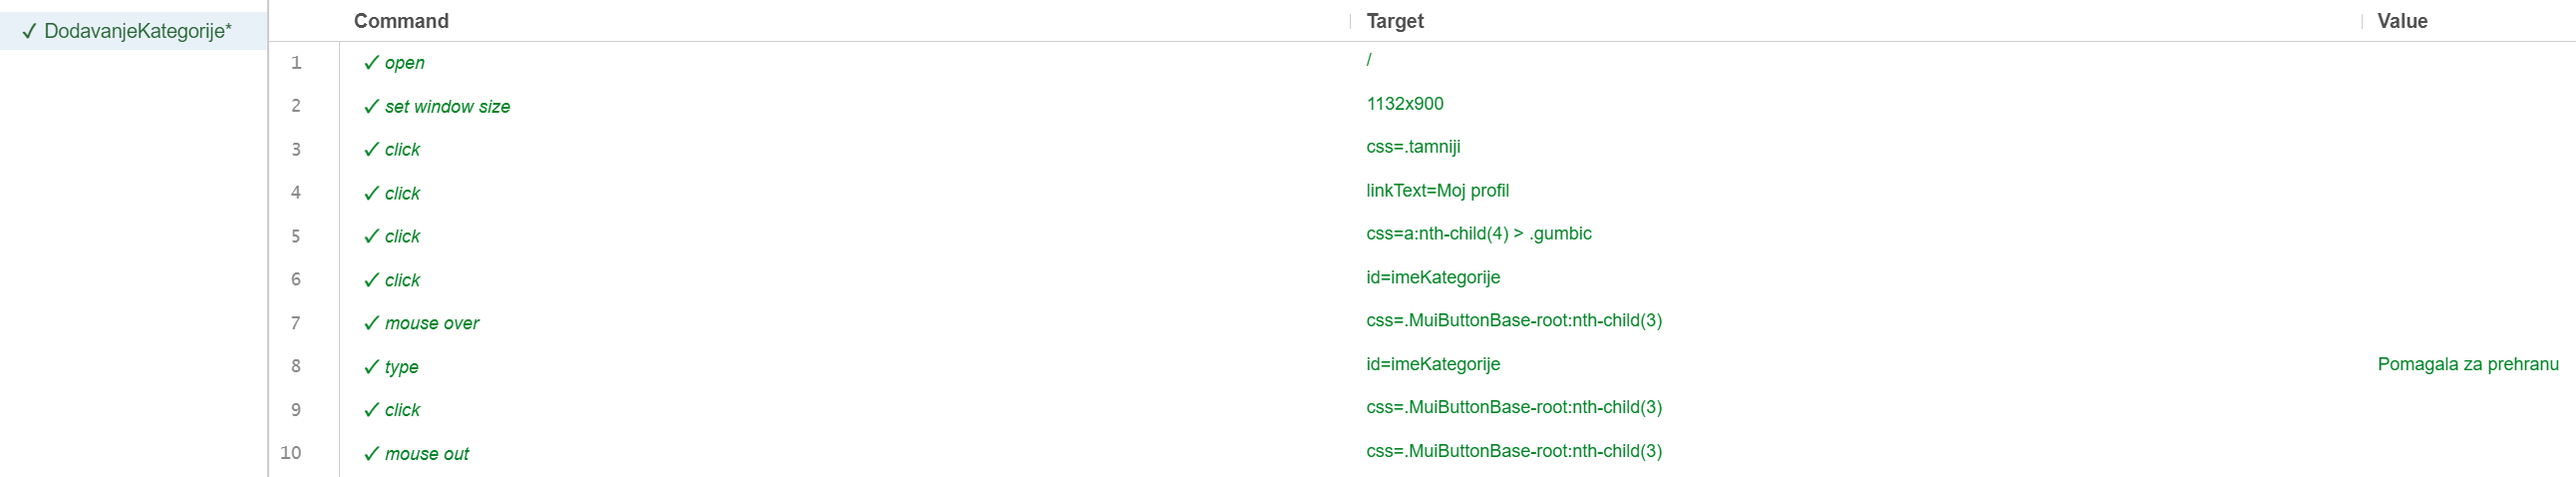
\includegraphics[scale=0.4]{slike/selenium5.png}}%
				\centering
				\caption{Akcije petog Selenium testa}
				\label{fig:selenium5}
			\end{figure}

                Uz pet do sada prikazanih Selenium testova, dodatno su testirane i funkcionalnosti stvaranja oglasa, dodavanja potkategorije i uređivanja podataka, ali zbog preglednosti i sažetosti ti testovi nisu uključeni u dokumentaciju. 

                \eject
			
			 %\textit{Potrebno je provesti i opisati ispitivanje sustava koristeći radni okvir Selenium\footnote{\url{https://www.seleniumhq.org/}}. 
			 %Razraditi \textbf{minimalno 4 ispitna slučaja} u kojima će se ispitati redovni slučajevi, 
			% rubni uvjeti te poziv funkcionalnosti koja nije implementirana/izaziva pogrešku kako bi se vidjelo na koji način sustav reagira kada nešto nije u potpunosti ostvareno. 
			 %Ispitni slučaj se treba sastojati od ulaza (npr. korisničko ime i lozinka), očekivanog izlaza ili rezultata, koraka ispitivanja i dobivenog izlaza ili rezultata.\\ }
			 
			 %\textit{Izradu ispitnih slučajeva pomoću radnog okvira Selenium moguće je provesti pomoću jednog od sljedeća dva alata:}
			 %\begin{itemize}
			 	%\item \textit{dodatak za preglednik \textbf{Selenium IDE} - snimanje korisnikovih akcija radi automatskog ponavljanja ispita	}
			 	%\item \textit{\textbf{Selenium WebDriver} - podrška za pisanje ispita u jezicima Java, C\#, PHP koristeći posebno programsko sučelje.}
			 %\end{itemize}
		 	%\textit{Detalji o korištenju alata Selenium bit će prikazani na posebnom predavanju tijekom semestra.}
			
			%\eject 
		
		
		\section{Dijagram razmještaja}
			
			%\textbf{\textit{dio 2. revizije}}

                Dijagram razmještaja opisuje konkretno ostvarenje odabrane arhitekture aplikacije - na slici 5.14 moguće je vidjeti raspodjelu programske potpore na konkretno sklopovlje. Kod za prikaz korisničkog sučelja i komunikaciju s korisnikom pisan u React.js pušten je u pogon na platformi Render. Kako bi aplikacija bila funkcionalna, u pogon su zasebno pušteni (engl. deployani) baza podataka ostvarena koristeći PostgreSQL te kod za poslovnu logiku i komunikaciju s bazom (backend) pisan u Java Spring Boot-u. Kako bi kod za backend bio uspješno deployan, za njega postoji i Docker container koji osigurava da je u njemu ispravno "spakiran" sav kod, kao i zavisnosti potrebne za uspješan rad istoga. I backend i baza podataka pušteni su u pogon koristeći platformu Render. \\

                Uz ovo, na platformi Firebase napravljen je Cloud Storage Bucket koji služi za jednostavnu pohranu slika potrebnih za uspješan prikaz oglasa. Komunikacija između zasebnih uređaja i platformi osigurana je protokolom HTTPS (komunikacija između klijentovog računala tj. web preglednika na istome i web poslužitelja deployanog na platformi Render, kao i komunikacija između web poslužitelja i Cloud Storage Bucket-a deployanog na platformi Firebase). Kako bi web poslužitelj korisniku mogao poslužiti sav potreban sadržaj, on komunicira s backendom koji po potrebi komunicira s bazom podataka.

                \begin{figure}[H]
				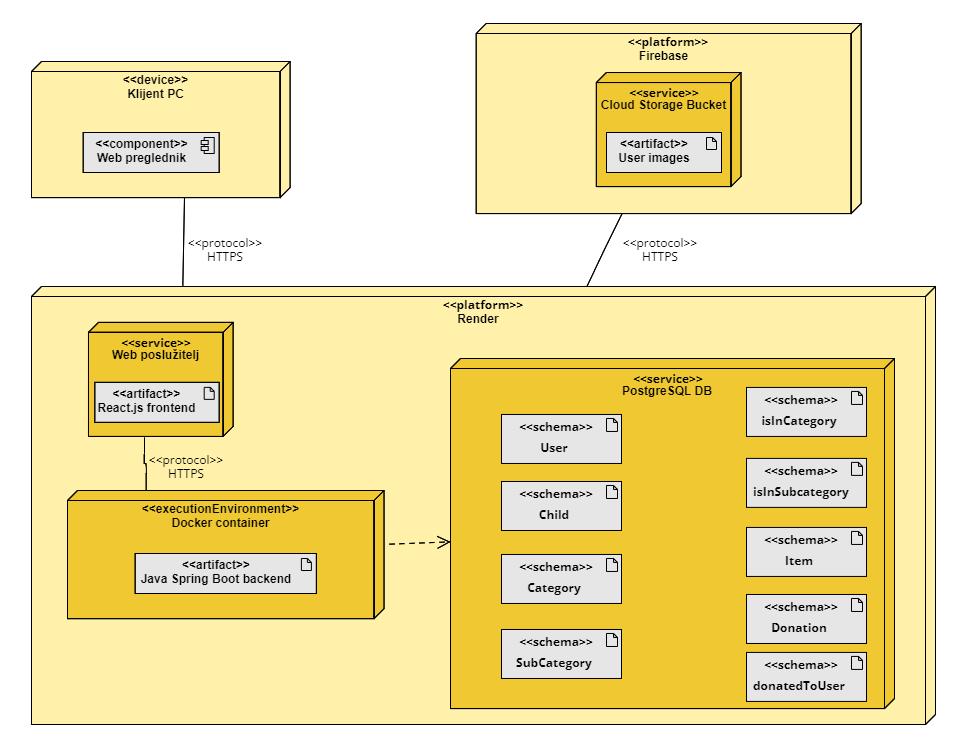
\includegraphics[width=\textwidth,height=0.8\textheight]{dijagrami/Dijagram razmjestajav2.png}
				\centering
				\caption{Dijagram razmještaja}
				\label{fig:DeploymentDiagram}
			\end{figure}
			
			\eject 
		
		\section{Upute za puštanje u pogon}
		
			%\textbf{\textit{dio 2. revizije}}\\
                Frontend, backend i baza podatka puštene su u pogon na platformi Render. Upute za pristupanje platformi Render, kao i upute za puštanje u pogon (engl. deploy) slijede u sljedećim sekcijama.
          
			    \subsection{Pristupanje Renderu}

                Kako bi pristupili Renderu, prilikom prijave u web aplikaciju koristimo GitLab račune koji se direktno mogu povezati s njime. Povezivanjem Gitlab računa s platformom Render dobivamo lakši pristup kodu koji će se pustiti u pogon.

                \begin{figure}[H]
				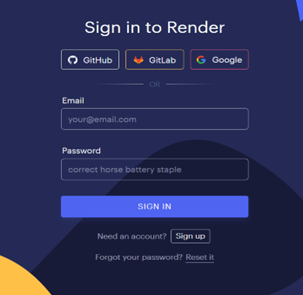
\includegraphics[width=0.6\textwidth,height=0.3\textheight]{slike/renderSignIn.png}
				\centering
				\caption{Render sign in}
				\label{fig:renderSignIn}
			\end{figure}

                \subsection{Backend deploy na Render}

                \textbf{1. Priprema}\\
                
                Prije puštanja aplikacije u pogon na Renderu potrebno je u izvorni kod za backend dodati Dockerfile za Maven projekt te u datoteci application.properties postaviti property server.servlet.context-path na /api da bude prefiks svim zahtjevima na backend.
			
			\eject 

                \textbf{2. Kreiranje baze podataka}\\

                U render dashboard potrebno je:

                \begin{itemize}
                    \item Pritisnuti tipku New te onda odabrati opciju PostgreSQL za kreiranje baze
                    \begin{figure}[H]
    			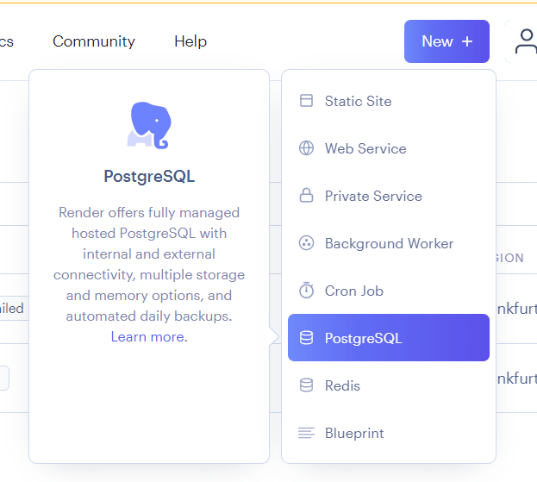
\includegraphics[width=0.6\textwidth,height=0.3\textheight]{slike/postgresqlCreate.png}
    			\centering
    			\caption{Kreiranje nove PostgreSQL baze}
    			\label{fig:newPostgreSQLDB}
    			\end{figure}
                    \item Postaviti ime baze
                    \item Database i User ostaviti prazno jer se automatski generira pri kreiranju baze
                    \item Postaviti Region na Frankfurt
                    \item Pritisnuti Create Database
                \end{itemize}

                \begin{figure}[H]
				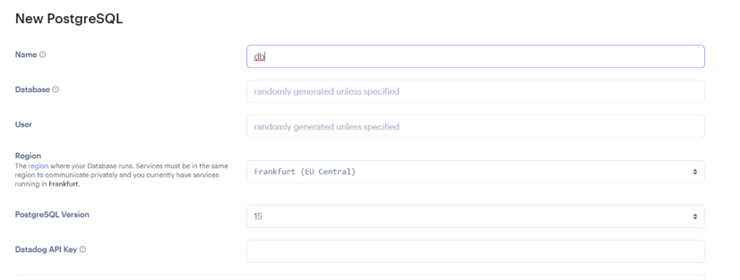
\includegraphics[width=0.8\textwidth,height=0.25\textheight]{slike/postgresqlNew.png}
				\centering
				\caption{Ispunjavanje podataka o bazi}
				\label{fig:postgresqlFillData}
			\end{figure}

                Prije puštanja backend-a u pogon, u datoteci application.properties moramo uvrstiti username, password za pristup bazi, database, hostname i port za url prema bazi na koju se treba spojiti.

                \begin{figure}[H]
				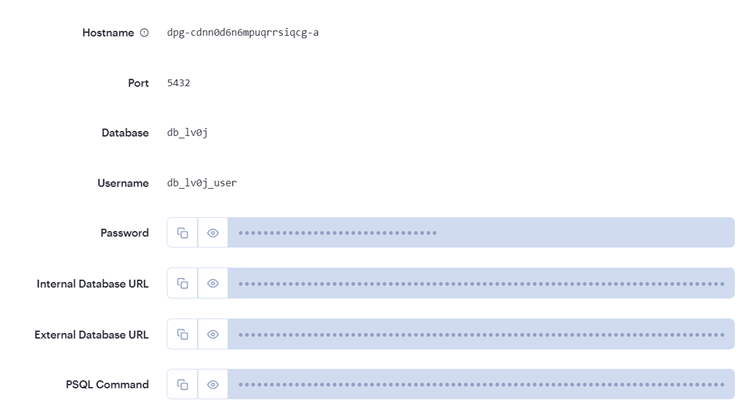
\includegraphics[width=0.8\textwidth,height=0.25\textheight]{slike/postgresqlNewFilled.png}
				\centering
				\caption{Ispunjavanje podataka u datoteci application.properties}
				\label{fig:applicationPropertiesDB}
			\end{figure}

                \textbf{3. Kreiranje backenda}\\

                U Render dashboard potrebno je:

                \begin{itemize}
                    \item Pritisnuti tipku New te onda odabrati opciju Web Service za kreiranje web usluge
                    \item Povezati GitLab račun - nakon povezivanja su za odabir dostupni svi projekti na koje imate prava pristupa
                    \item Pritisnuti Connect pokraj odgovarajućeg projekta
                    \begin{figure}[H]
    			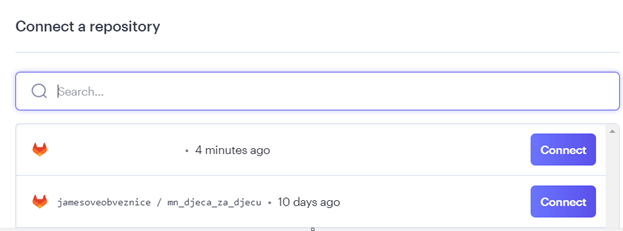
\includegraphics[width=0.8\textwidth,height=0.25\textheight]{slike/connectRepo.png}
    			\centering
    			\caption{Povezivanje repozitorija}
    			\label{fig:connectRepo}
    			\end{figure}
                    \item Postaviti ime za servis (ime servisa na kraju će biti dio web adrese)
                    \item Root directory postaviti na IzvorniKod/backend
                    \item Environment postaviti na Docker
                    \item Region postaviti na Frankfurt
                    \begin{figure}[H]
    			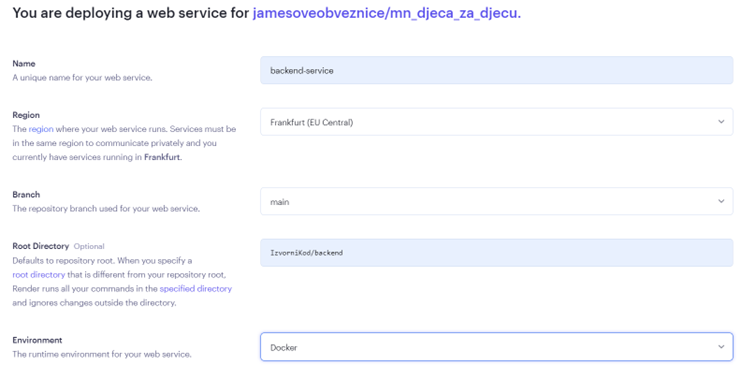
\includegraphics[width=0.8\textwidth,height=0.25\textheight]{slike/deployWebService.png}
    			\centering
    			\caption{Podaci za puštanje web servisa u pogon}
    			\label{fig:deployWebService}
    			\end{figure}
                    \item Na dnu proširiti \textit{advanced}
                    \item Postaviti putanju za Dockerfile ovisno koji se package manager koristi (u ovom slučaju putanja je ./docker/maven/Dockerfile)
                    \begin{figure}[H]
                    \makebox[\textwidth][c]{
\includegraphics[]{slike/dockerfilePath.png}}%
    			\centering
    			\caption{Putanja Dockerfile-a}
    			\label{fig:dockerFilePath}
    			\end{figure}
                    \item Pritisnuti Create Web Service
                \end{itemize}

                Nakon izvođenja svih ovih koraka, u pogon bi se trebala uspješno pustiti (eng. deployati) backend aplikacija. Nakon puštanja backend aplikacije u pogon, isto ćemo napraviti i za frontend aplikaciju.

                \eject

                \subsection{Frontend deploy na Render}

                Kako bi se frontend uspješno pustio u pogon, u Render dashboard potrebno je:

                \begin{itemize}
                    \item Pritisnuti tipku New i odabrati opciju Web Service za kreiranje web usluge
                    \item Povezati GitLab račun - nakon povezivanja su za odabir dostupni svi projekti na koje imate prava pristupa
                    \item Pritisnuti Connect pokraj odgovarajućeg projekta
                    \begin{figure}[H]
    			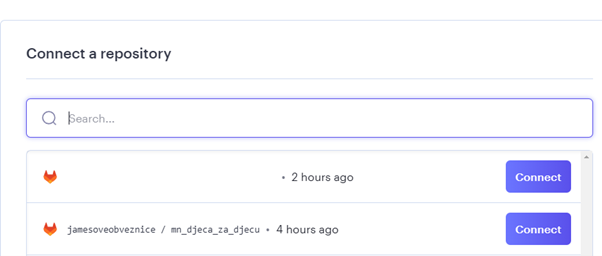
\includegraphics[width=\textwidth,height=0.25\textheight]{slike/connectFront.png}
    			\centering
    			\caption{Povezivanje repozitorija za frontend}
    			\label{fig:connectRepoFront}
    			\end{figure}
                    \item Postaviti ime za servis (ime servisa na kraju će biti dio web adrese)
                    \item Root directory postaviti na IzvorniKod/Frontend/dzd-app/
                    \item Environment postaviti na Node
                    \begin{figure}[H]
    			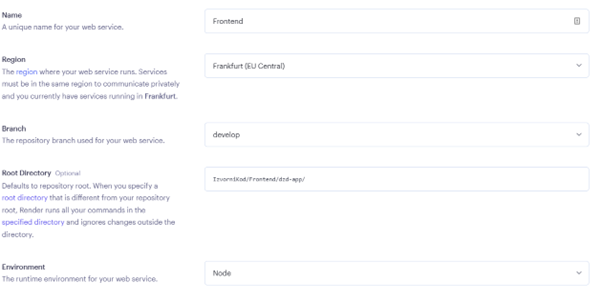
\includegraphics[scale=0.75]{slike/fillDataDeployFront.png}
    			\centering
    			\caption{Ispunjavanje podataka o frontendu}
    			\label{fig:fillDataFront}
    			\end{figure}
                    \item Region postaviti na Frankfurt
                    \item Odabrati branch iz kojeg se uzimaju datoteke za frontend
                    \item Build Command postaviti na yarn build
                    \item Start Command postaviti na yarn start-prod
                    \begin{figure}[H]
    			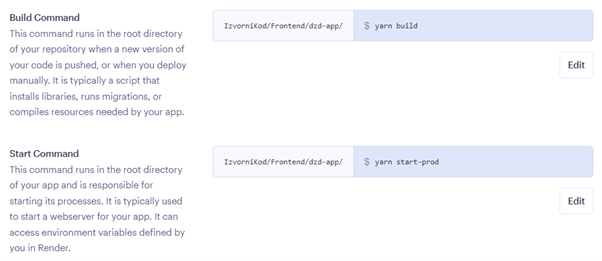
\includegraphics[]{slike/buildFront.png}
    			\centering
    			\caption{Unošenje ispravnih naredbi}
    			\label{fig:buildFrontCommands}
    			\end{figure}\textbf{}
                    \item Na dnu pritisnuti Advanced
                    \item Dodati potrebne Environment varijable - API\_BASE\_URL postaviti na adresu deployanog backenda aplikacije dostupnu na Render dashboardu
                    \item Isključiti Auto-Deploy kako se projekt ne bi ponovno deployao za svaki novi commit
                    \item Pritisnuti Create Web Service
                \end{itemize}

                Nakon izvođenja svih ovih koraka, u pogon bi se trebala uspješno pustiti (eng. deployati) frontend aplikacija. Stranici pristupamo preko URL-a za \underline{frontend}\footnote{\url{https://frontend-service-3f78.onrender.com/}}.